\documentclass[11pt,a4paper]{article}
\usepackage[T1]{fontenc}
\usepackage[utf8]{inputenc}
\usepackage{lmodern}
\usepackage{microtype}
\usepackage[a4paper,margin=25mm,headheight=14pt]{geometry}
\usepackage[numbers,sort&compress]{natbib}
\usepackage{amsmath,amssymb}
\usepackage{booktabs}
\usepackage{longtable}
\usepackage{multirow}
\usepackage{graphicx}
\usepackage[font=small,labelfont=bf]{caption}
\usepackage{enumitem}
\usepackage{xcolor}
\usepackage{tikz}
\usetikzlibrary{arrows.meta,positioning}
\usepackage{fancyhdr}
\usepackage{lastpage}
\usepackage{hyperref}
\usepackage[nameinlink,noabbrev]{cleveref}
\hypersetup{colorlinks=true,linkcolor={blue!50!black},citecolor={blue!50!black},urlcolor={blue!50!black}}
\captionsetup[figure]{name=Fig.}
\setlist{nosep}
\graphicspath{{../results/figures/}}
\newcommand{\clr}{\operatorname{clr}}
\newcommand{\ox}[1]{\ensuremath{\mathrm{#1}}}
\pagestyle{fancy}
\fancyhf{}
\lhead{\small Composition analysis and classification of ancient glass}
\rhead{\small Page \thepage\ of \pageref*{LastPage}}
\renewcommand{\headrulewidth}{0.4pt}

\begin{document}

%% ================================================================== Summary
\thispagestyle{empty}
\begin{center}
{\LARGE\bfseries Composition Analysis and Classification\\[3pt] of Ancient Glass Artefacts\par}
\vspace{6pt}
{\normalsize Xiangyu Luo\par}
{\small CUMCM 2022 Problem C; undergraduate mathematical modelling training, Southwest Petroleum University (2023)\par}
\vspace{10pt}
{\Large\bfseries Summary\par}
\end{center}

\noindent
Archaeologists have classified 58 ancient Chinese glass artefacts as high-potassium (high-K) or lead--barium (Pb--Ba) glass and have measured 14 oxides at 69 surface points; eight further artefacts are unclassified.
Burial weathering alters the measured composition and so obscures both the statistical regularities of each glass type and its identification.
Because the oxide percentages of a point sum to about 100\%, we analyse them as compositional data in centred log-ratio (clr) coordinates, and because several points can come from one artefact, we test artefact attributes on artefacts and validate every model by leaving whole artefacts out.

For Problem 1, exact contingency tests show that weathering is associated with glass type (Fisher $p=0.011$; 70\% of Pb--Ba against 33\% of high-K artefacts).
Decoration appears unrelated in the pooled table ($p=0.10$), but stratifying by type reveals that the six weathered high-K artefacts are exactly the six decoration-B artefacts ($p=5\times10^{-5}$), whereas decoration and weathering are unrelated within Pb--Ba glass; colour shows no association in either type.
Weathering raises \ox{SiO_2} from a median 65.5\% to 93.5\% in high-K glass by leaching \ox{K_2O} and \ox{Al_2O_3}, and in Pb--Ba glass it lowers \ox{SiO_2} from 54.6\% to 25.0\% while enriching PbO and \ox{P_2O_5}.
To predict the pre-weathering composition we treat weathering as a perturbation in clr space with artefact-specific noise and derive the best linear predictor, a calibrated shift whose gains shrink the most variable parts towards the unweathered mean.
On the two artefacts with both weathered and unweathered spots it reduces the error of the major oxides from 7.3 and 8.1 to 3.4 and 4.6 percentage points, and 23 of 26 corrected Pb--Ba points fall inside the observed range of unweathered glass, against 16 for an uncalibrated shift.

For Problem 2, the single variable PbO+BaO separates the types with a margin of ten percentage points (high-K $\le4.27\%$, Pb--Ba $\ge14.34\%$), which a classification tree, a random forest and a log-ratio logistic model confirm in leave-one-artefact-out validation (67, 67 and 66 of 67 points).
Ward clustering of weathering-corrected log-ratios divides Pb--Ba glass into four sub-classes (barium-free, copper-free, low-impurity and impurity-bearing) that k-means reproduces exactly and that withstand 10\% measurement noise (adjusted Rand index 0.91), although the gap statistic shows that they partition a graded continuum rather than separated groups; high-K glass has no sub-class structure supported by the data.

For Problem 3, the rule, the logistic model and an Aitchison-distance classifier all assign A1, A6 and A7 to high-K and A2, A3, A4, A5 and A8 to Pb--Ba, unchanged under 40\% multiplicative noise and across all detection-limit and regularisation settings; A2 falls in the barium-free sub-class and the other four in the impurity-bearing sub-class.

For Problem 4, clr correlations with false-discovery-rate control give two significant associations within high-K glass and five within Pb--Ba glass, and two of 55 pairs differ between the types, most clearly \ox{Fe_2O_3}--CuO, which is positive in high-K and negative in Pb--Ba glass.

\medskip
\noindent\textbf{Keywords:} compositional data; centred log-ratio; stratified exact tests; calibrated weathering correction; Ward clustering; gap statistic; sensitivity analysis

\newpage
\setcounter{tocdepth}{2}
\tableofcontents
\newpage

%% ================================================================== 1
\section{Introduction}

\subsection{Problem Background}
Glass is an important material witness of early exchange along the Silk Road.
Glass beads made in West Asia and Egypt reached China in the Warring States period, after which glass was also produced locally from local raw materials, so that imported and domestic glass can look alike while differing in chemical composition \citep{gan2009}.
The main raw material of glass is quartz sand, that is, \ox{SiO_2}.
Because pure silica melts at a very high temperature, a flux is added, and the choice of flux defines the glass system: plant ash, natron or saltpetre introduce alkali oxides, whereas lead ore introduces PbO and, in the Chinese tradition, BaO.
Limestone, which becomes CaO on firing, is added as a stabiliser.
Pb--Ba glass, rich in PbO and BaO, is generally regarded as a Chinese invention, while high-K glass, fluxed with potassium-rich materials such as plant ash, was widespread in Lingnan, South-East Asia and India \citep{gan2009}.

Ancient glass is vulnerable to its burial environment.
Water and soil exchange ions with the glass surface, so that some components are leached and others are deposited, and the composition measured on a weathered surface can differ greatly from that of the original glass.
A high-K glass whose potassium has been leached, or a Pb--Ba glass whose silica has been depleted, may then be misjudged, which is why the analysis of composition, the correction for weathering and the identification of glass type have to be treated together.

\subsection{Restatement of the Problem}
The contest data consist of three sheets.
Sheet~1 lists 58 artefacts with their decoration (A, B or C), glass type, colour and surface weathering; sheet~2 gives the oxide percentages of the sampling points of these artefacts, where a blank cell means that the oxide was not detected; and sheet~3 gives the compositions and weathering status of eight unclassified artefacts.
A point is valid if its oxide percentages sum to between 85\% and 105\%.

The first problem asks how surface weathering is related to glass type, decoration and colour, how the composition of each type differs with and without weathering, and what the composition of each weathered point was before weathering.
The second asks for the rule that separates high-K from Pb--Ba glass, for a division of each type into sub-classes on suitable oxides, and for an analysis of the rationality and sensitivity of that division.
The third asks for the type of each unclassified artefact together with the sensitivity of the assignment, and the fourth asks for the associations between oxides within each type and for the differences between the types.

\subsection{Literature Review}
Oxide percentages are compositional data: they carry only relative information and are constrained to a constant sum.
\citet{aitchison1986} showed that the usual statistics of raw percentages are distorted by this constraint, because an increase of one part forces the others to decrease, and he proposed to analyse compositions through log-ratios, which map the simplex onto a Euclidean space in which means, distances and correlations are meaningful.
The geometry was later formalised, with perturbation as the natural operation for changes of composition \citep{pawlowsky2015}.
Zeros, which here arise from oxides below the detection limit, have to be replaced before log-ratios can be taken; multiplicative replacement keeps the ratios of the detected parts unchanged \citep{martin2003}.

Contest solutions of this problem typically combine chi-square tests for the association questions, ratio or regression models for the pre-weathering composition, decision trees, random forests or logistic regression for the type rule, k-means for the sub-classes and Spearman or grey relational analysis for the associations between oxides.
Two issues recur in these approaches: raw percentages are used without regard to closure, and the sampling points are treated as independent observations although several points may come from one artefact.
Our models are built to avoid both, and we add stratified analysis, validation on paired spots, cluster-validity tests and a systematic sensitivity analysis, using exact tests \citep{agresti2002}, hierarchical clustering \citep{ward1963}, silhouettes \citep{rousseeuw1987}, the gap statistic \citep{tibshirani2001} and the adjusted Rand index \citep{hubert1985}.

\subsection{Overview of Our Work}
\Cref{fig:flow} summarises the work.
After preprocessing, which screens invalid points, replaces non-detects and transforms the compositions to clr coordinates, Problem~1 is solved with exact tests on artefacts, non-parametric comparisons of composition and a calibrated perturbation model of weathering.
The weathering correction feeds Problem~2, whose type rule and sub-classes are reused in Problem~3, and the corrected log-ratios are the input of the correlation analysis of Problem~4.
A common sensitivity analysis then varies the detection-limit replacement, the correction model and the regularisation of the classifier.

\begin{figure}[ht]
\centering
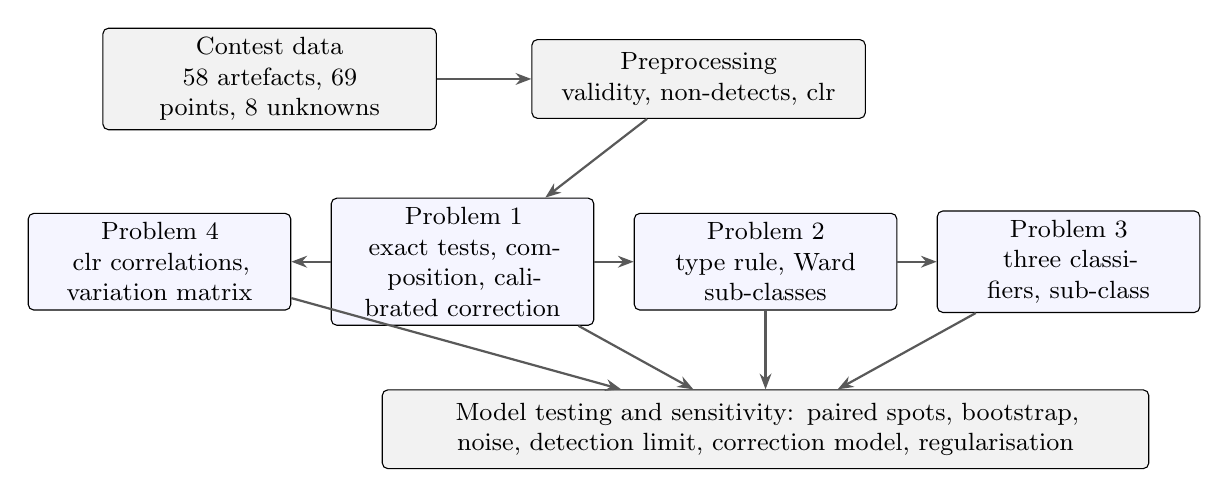
\begin{tikzpicture}[
  box/.style={draw,rounded corners=2pt,align=center,font=\small,minimum height=10mm,text width=31mm,fill=blue!4},
  pre/.style={box,fill=gray!10,text width=40mm},
  arr/.style={-{Stealth[length=2mm]},thick,gray!70!black},
  node distance=6mm and 5mm]
\node[pre] (data) {Contest data\\58 artefacts, 69 points, 8 unknowns};
\node[pre,right=12mm of data] (prep) {Preprocessing\\validity, non-detects, clr};
\node[box,below left=10mm and -8mm of prep] (q1) {Problem 1\\exact tests, composition, calibrated correction};
\node[box,right=of q1] (q2) {Problem 2\\type rule, Ward sub-classes};
\node[box,right=of q2] (q3) {Problem 3\\three classifiers, sub-class};
\node[box,left=of q1] (q4) {Problem 4\\clr correlations, variation matrix};
\node[pre,below=10mm of q2,text width=95mm] (sens) {Model testing and sensitivity: paired spots, bootstrap, noise, detection limit, correction model, regularisation};
\draw[arr] (data) -- (prep);
\draw[arr] (prep) -- (q1);
\draw[arr] (q1) -- (q2);
\draw[arr] (q2) -- (q3);
\draw[arr] (q1) -- (q4);
\draw[arr] (q1) -- (sens);
\draw[arr] (q2) -- (sens);
\draw[arr] (q3) -- (sens);
\draw[arr] (q4) -- (sens);
\end{tikzpicture}
\caption{Structure of the work.}\label{fig:flow}
\end{figure}

%% ================================================================== 2
\section{Assumptions and Justifications}\label{sec:assumptions}

The models rest on five assumptions, each stated with its justification.
\begin{enumerate}[label=A\arabic*.,leftmargin=*,itemsep=4pt]
\item \emph{A sampling point has the weathering status of its artefact, except for the points marked as unweathered or severely weathered spots in sheet~2.} The problem statement defines the points in this way.
\item \emph{A blank cell means that the oxide was below the detection limit.} The problem statement says so; for log-ratio analysis such values are replaced by half of the reporting step of 0.01\%, and \cref{sec:sens} shows how the results depend on this choice.
\item \emph{Weathering acts on the clr coordinates of a composition as a type-specific average shift plus an artefact-specific deviation that is independent of the unweathered composition.} Leaching and deposition change parts multiplicatively, which is a shift in clr coordinates; the deviation absorbs differences in burial time and environment, which cannot be observed for individual artefacts.
\item \emph{Different artefacts are independent observations, whereas points of the same artefact are not.} Points of one artefact share its recipe and its burial history.
\item \emph{The type labels of sheet~1 are correct.} They were assigned by archaeologists from chemical and other evidence, and \cref{sec:q2} shows that they are consistent with a simple chemical rule.
\end{enumerate}

%% ================================================================== 3
\section{Notations}\label{sec:notation}

The symbols used throughout the paper are listed below; others are defined where they appear.

\begin{center}
\small
\begin{tabular}{ll}
\toprule
Symbol & Meaning \\
\midrule
$x\in\mathbb{R}^{14}_{>0}$ & composition of a sampling point (wt\%, closed to 100\%) \\
$\clr(x)$, $z$ & centred log-ratio coordinates of a composition \\
$\delta$ & replacement value for undetected oxides (0.005\%) \\
$w$, $u$ & weathered composition and its unweathered state \\
$t\in\{\text{high-K},\text{Pb--Ba}\}$ & glass type \\
$\mu_{u,t}$, $\mu_{w,t}$ & mean clr coordinates of unweathered and weathered points of type $t$ \\
$\Delta_t$ & average weathering shift of type $t$ in clr coordinates \\
$b_{t,j}$ & calibration gain of part $j$ for type $t$ \\
$d_A(x,y)$ & Aitchison distance $\lVert\clr(x)-\clr(y)\rVert_2$ \\
$k$ & number of sub-classes \\
$\varepsilon$ & relative size of multiplicative perturbations \\
ARI & adjusted Rand index between two partitions \\
$\tau_{ij}$ & variance of the log-ratio $\log(x_i/x_j)$ \\
$r$, $n$ & correlation coefficient, number of points \\
\bottomrule
\end{tabular}
\end{center}

%% ================================================================== 4
\section{Data Description and Preprocessing}\label{sec:data}

\subsection{Structure of the Data}
Sheet~1 contains 18 high-K and 40 Pb--Ba artefacts.
Decoration B occurs only on high-K glass, where each of the three decorations is represented by six artefacts, whereas the Pb--Ba artefacts carry decoration A (16) or C (24).
Colour takes eight values and is missing for four Pb--Ba artefacts, and 34 artefacts are weathered.
Sheet~2 lists 69 sampling points.
Most artefacts contribute one point, some contribute two parts of the same object, nine points are unweathered spots taken on weathered artefacts and three are severely weathered spots; by assumption~A1, all other points inherit the weathering status of their artefact.
The data are therefore nested, with points within artefacts, and this nesting decides the unit of each analysis below.

\subsection{Validity Screening}
The validity rule of the problem removes points 15 and 17, whose totals of 79.5\% and 71.9\% are far below 85\%, and leaves 67 valid points, 18 of high-K and 49 of Pb--Ba glass, of which 35 are unweathered and 32 weathered.
The totals of the valid points range from 88.4\% to 100.0\%; the shortfall consists of unmeasured components such as water and carbonates, and since only relative information is used below, every composition is closed to 100\% before analysis.

\subsection{Non-Detects and the Log-Ratio Transform}
Of the $67\times14$ cells, many are blank, and blanks are frequent for the trace oxides \ox{Na_2O}, \ox{SnO_2} and \ox{SO_2} and for the flux oxides of the other type (\cref{tab:compfull} in the appendix gives the detection rates).
For log-ratio analysis, undetected oxides are replaced by $\delta=0.005\%$, half the reporting step, and the composition is re-closed; this multiplicative replacement leaves the ratios between detected parts unchanged \citep{martin2003}.
For a composition $x$ with $D=14$ parts, the centred log-ratio transform and its inverse are
\begin{equation}\label{eq:clr}
\clr(x)_j = \log x_j - \frac{1}{D}\sum_{i=1}^{D}\log x_i ,\qquad
\clr^{-1}(z) = \mathcal{C}\big(e^{z_1},\dots,e^{z_D}\big),
\end{equation}
where $\mathcal{C}$ denotes closure to 100\%.
The clr coordinates sum to zero, and Euclidean operations on them correspond to the Aitchison geometry of the simplex: the difference of two clr vectors describes the relative change between two compositions, and its norm is the Aitchison distance $d_A$ \citep{aitchison1986,pawlowsky2015}.

The practical consequence is large.
Within Pb--Ba glass, for example, the raw percentages of \ox{SiO_2} and PbO have a correlation of $-0.74$, which mostly expresses the fact that two major parts of a closed sum must trade off, whereas their clr coordinates have a correlation of $+0.61$ and their log-ratio has the smallest variance of all pairs (\cref{sec:q4}).
Statements about associations and distances are therefore made in clr coordinates throughout, and raw percentages are used only where a rule must be read directly from a measurement.

%% ================================================================== 5
\section{Model I: Weathering and Its Effect on Composition (Problem 1)}\label{sec:q1}

\subsection{Association of Weathering with Type, Decoration and Colour}

\subsubsection{Model}
Weathering status, type, decoration and colour are attributes of artefacts, so the association analysis uses the 58 artefacts of sheet~1 and not the 67 points, which would count some artefacts twice.
For each attribute we form the contingency table of attribute level against weathering and measure association with the Pearson statistic $\chi^2=\sum_{ij}(O_{ij}-E_{ij})^2/E_{ij}$ and with Cram\'er's $V=\sqrt{\chi^2/(n(\min(r,c)-1))}$.
The asymptotic $\chi^2$ distribution is unreliable here, because a third of the expected counts of the decoration table and three quarters of those of the colour table are below five.
We therefore use exact tests: Fisher's exact test for $2\times2$ tables, which conditions on the margins and refers the table to the hypergeometric distribution, and for larger tables a Monte Carlo exact test that permutes the weathering labels with fixed margins 20{,}000 times \citep{agresti2002}.

Because decoration B occurs only on high-K glass and the types weather at different rates, a pooled table can mix the effect of decoration with that of type.
We therefore repeat the tests within each type and combine the strata in a stratified permutation test whose statistic is the sum of the within-type $\chi^2$ values and whose permutations exchange weathering labels only within a type.
This test asks whether decoration or colour is related to weathering once type is held fixed.

\subsubsection{Results}
\Cref{tab:assoc} shows the pooled results.
Weathering is associated with type: 28 of 40 Pb--Ba artefacts (70\%) but only 6 of 18 high-K artefacts (33\%) are weathered, so the odds of weathering are 4.7 times higher for Pb--Ba glass (Fisher $p=0.011$, $V=0.34$).
In the pooled table neither decoration ($p=0.10$) nor colour ($p=0.59$) is significantly associated with weathering.

\begin{table}[ht]
\centering
\caption{Association of surface weathering with artefact attributes. Pooled tests use all artefacts; stratified tests permute weathering labels within each glass type.}\label{tab:assoc}
\small
\begin{tabular}{llrrrrl}
\toprule
Stratum & Attribute & $n$ & $\chi^2$ & exact $p$ & $V$ & test \\
\midrule
All & type & 58 & 6.88 & 0.011 & 0.34 & Fisher \\
All & decoration & 58 & 4.96 & 0.104 & 0.29 & Monte Carlo \\
All & colour & 54 & 6.29 & 0.586 & 0.34 & Monte Carlo \\
\addlinespace
High-K & decoration & 18 & 18.00 & $<0.001$ & 1.00 & Monte Carlo \\
High-K & B versus A/C & 18 & 18.00 & $5.4\times10^{-5}$ & 1.00 & Fisher \\
High-K & colour & 18 & 4.50 & 0.317 & 0.50 & Monte Carlo \\
Pb--Ba & decoration & 40 & 0.02 & 1.000 & 0.02 & Fisher \\
Pb--Ba & colour & 36 & 9.00 & 0.248 & 0.50 & Monte Carlo \\
\addlinespace
Within type & decoration & 58 & 18.02 & $<0.001$ & -- & stratified \\
Within type & colour & 54 & 13.50 & 0.168 & -- & stratified \\
\bottomrule
\end{tabular}
\end{table}

The stratified analysis changes the picture for decoration.
Within high-K glass, all six decoration-B artefacts are weathered and none of the twelve artefacts with decoration A or C is, so decoration and weathering coincide completely; under the null hypothesis of no association, the probability of this split is $1/\binom{18}{6}=5.4\times10^{-5}$.
Within Pb--Ba glass, by contrast, decoration A and C are weathered at almost the same rate (11 of 16 and 17 of 24, $p=1.00$).
The pooled test misses the high-K association because decoration B is a small group of six and because the many weathered decoration-C artefacts of Pb--Ba glass dilute the contrast between decorations.
Colour remains unrelated to weathering within each type ($p=0.32$ and $0.25$).

The association between decoration B and weathering cannot be interpreted causally from these data.
Decoration B may mark a production batch, a burial context or a find site, any of which could explain why these six artefacts are weathered, and since decoration B is never unweathered, the data cannot separate its effect from that of weathering itself.
This confounding matters again in \cref{sec:pred}, because the weathering effect of high-K glass is estimated by comparing decoration-B artefacts with the others.

\subsection{Statistical Regularities of Composition}

\subsubsection{Model}
The composition question concerns sampling points, since each point is a measurement of a surface.
Within each type, we compare unweathered and weathered points oxide by oxide with the two-sided Mann--Whitney test, which needs no normality and is robust to the many values at the detection limit, and adjust the 14 $p$-values of each type with Holm's method \citep{holm1979}.
Because many oxides are skewed or partly undetected, we summarise them by medians and detection rates.
As a multivariate complement, we compare the clr centres of unweathered and weathered points by the squared distance $\lVert\mu_{u,t}-\mu_{w,t}\rVert^2$ and assess it with 10{,}000 permutations of the weathering labels within the type.

\subsubsection{Results}
\Cref{tab:comp} and \cref{fig:box} show that weathering acts in opposite directions in the two types.
In high-K glass it removes the flux and the network modifiers: \ox{K_2O} falls from a median 9.83\% to 0.67\%, \ox{Al_2O_3} from 6.19\% to 1.72\%, and CaO, MgO and \ox{Fe_2O_3} also decrease, so that the weathered surface is nearly pure silica with a median \ox{SiO_2} of 93.5\% against 65.5\% before weathering.
This is the pattern expected from the leaching of alkali ions, which leaves a silica-rich layer behind.
In Pb--Ba glass, the weathered surface instead loses silica, with \ox{SiO_2} falling from 54.6\% to 25.0\%, while PbO rises from 20.1\% to 44.1\%, \ox{P_2O_5} from 0.19\% to 4.97\% and CaO from 0.84\% to 2.88\%.
The enrichment of lead together with phosphorus and calcium suggests that lead is retained, probably as phosphate and carbonate phases formed with components supplied by the burial soil, while silica is removed.
BaO, in contrast, changes little (8.99\% and 8.79\%), so the ratio of PbO to BaO is itself an indicator of weathering in Pb--Ba glass.

\begin{table}[ht]
\centering
\caption{Median composition (wt\%) of the valid points by type and weathering; $p$ is the Holm-adjusted Mann--Whitney $p$-value (14 oxides per type). Oxides with adjusted $p<0.1$ in at least one type are shown; \cref{tab:compfull} gives all oxides with detection rates.}\label{tab:comp}
\small
\begin{tabular}{lrrrrrr}
\toprule
& \multicolumn{3}{c}{High-K (12 U / 6 W)} & \multicolumn{3}{c}{Pb--Ba (23 U / 26 W)}\\
\cmidrule(lr){2-4}\cmidrule(lr){5-7}
Oxide & unweathered & weathered & $p$ & unweathered & weathered & $p$ \\
\midrule
\ox{SiO_2} & 65.53 & 93.50 & 0.002 & 54.61 & 25.02 & $<0.001$ \\
\ox{K_2O} & 9.83 & 0.67 & 0.050 & 0.15 & 0.00 & 0.879 \\
CaO & 6.10 & 0.83 & 0.249 & 0.84 & 2.88 & 0.023 \\
\ox{Al_2O_3} & 6.19 & 1.72 & 0.003 & 3.86 & 2.38 & 0.218 \\
PbO & 0.15 & 0.00 & 0.249 & 20.12 & 44.06 & $<0.001$ \\
\ox{P_2O_5} & 1.02 & 0.28 & 0.163 & 0.19 & 4.97 & 0.002 \\
\bottomrule
\end{tabular}
\end{table}

\begin{figure}[ht]
\centering
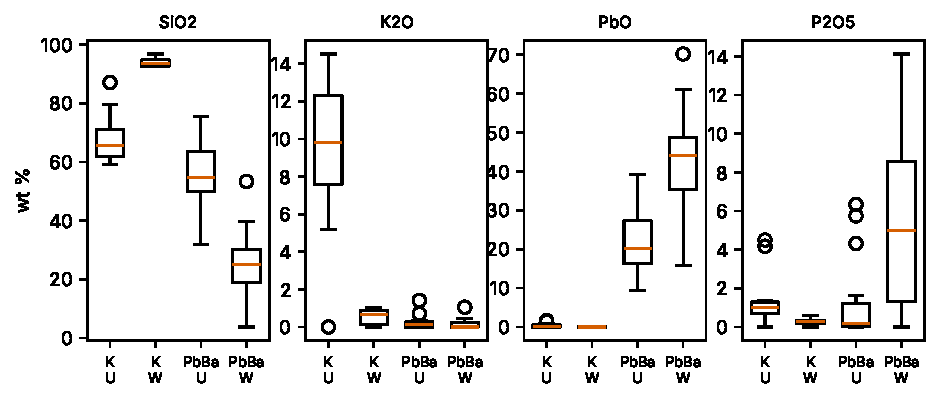
\includegraphics[width=\textwidth]{q1_boxplots}
\caption{Four oxides by type (K: high-K, PbBa: lead--barium) and weathering (U: unweathered, W: weathered) for the 67 valid points.}\label{fig:box}
\end{figure}

The multivariate test agrees for Pb--Ba glass, whose clr centres are 4.10 Aitchison units apart ($p<0.001$).
For high-K glass the centres are a similar 3.92 units apart, but the difference is not significant ($p=0.19$).
The reason is the small group of six weathered points combined with the large spread of the clr coordinates of trace oxides, which are often near the detection limit and therefore have log-ratios dominated by the replacement value.
The high-K weathering effect is thus clear in the major oxides, where \ox{SiO_2} and \ox{Al_2O_3} remain significant after Holm adjustment, but is estimated with much more uncertainty than the Pb--Ba effect as a whole composition.

\subsection{Prediction of the Pre-Weathering Composition}\label{sec:pred}

\subsubsection{Perturbation Model of Weathering}
Assumption~A3 states that a weathered composition $w$ of type $t$ and its unweathered state $u$ are related by
\begin{equation}\label{eq:model}
\clr(w) = \clr(u) - \Delta_t + e, \qquad \mathbb{E}[e]=0,\quad \operatorname{Cov}(e)=\Sigma_{e,t},\quad e\perp u,
\end{equation}
where $\Delta_t$ is the average weathering shift and $e$ the deviation of an individual artefact, caused for example by a longer burial or a wetter soil.
In the original composition this is a perturbation, $w = u\ominus\clr^{-1}(\Delta_t)\oplus\clr^{-1}(e)$, that is, every part is multiplied by a factor and the result is re-closed, which is the natural description of leaching and enrichment.
Since unweathered and weathered points of the same artefact are rarely available, we estimate the model from the two groups of points.
Taking expectations in \cref{eq:model} gives $\Delta_t=\mu_{u,t}-\mu_{w,t}$, estimated by the difference of the group means,
\begin{equation}\label{eq:shift}
\hat\Delta_t = \bar z_{u,t} - \bar z_{w,t}, \qquad \hat u_{\text{shift}} = \clr^{-1}\!\big(\clr(w) + \hat\Delta_t\big).
\end{equation}

The plain shift of \cref{eq:shift} would be optimal if every artefact weathered by exactly the average amount, but the deviation $e$ makes $\clr(w)$ a noisy measurement of $\clr(u)$.
The best linear predictor of $\clr(u)$ given $\clr(w)$ under \cref{eq:model} is
\begin{equation}\label{eq:blp}
\hat z_u = \mu_{u,t} + \Sigma_{u,t}\,(\Sigma_{u,t}+\Sigma_{e,t})^{-1}\big(\clr(w)-\mu_{w,t}\big),
\end{equation}
because $\operatorname{Cov}(\clr(u),\clr(w))=\Sigma_{u,t}$ and $\operatorname{Cov}(\clr(w))=\Sigma_{u,t}+\Sigma_{e,t}=\Sigma_{w,t}$.
This is the classical regression calibration of a variable measured with error \citep{fuller1987}.
With 6 or 26 weathered points the full covariance matrices cannot be estimated reliably, so we use their diagonals, which reduces \cref{eq:blp} to a gain for each part,
\begin{equation}\label{eq:gain}
\hat z_{u,j} = \bar z_{u,t,j} + b_{t,j}\big(\clr(w)_j - \bar z_{w,t,j}\big), \qquad b_{t,j}=\min\!\Big(1,\ \frac{s^2_{u,t,j}}{s^2_{w,t,j}}\Big),
\end{equation}
where $s^2$ denotes sample variances, and the cap at one reflects that the weathering noise cannot have negative variance.
Since $\clr^{-1}$ ignores additive constants, the prediction is a valid composition without further adjustment.
A gain of one reproduces the plain shift, whereas a small gain indicates that the weathered value of a part varies much more than the unweathered value and therefore says little about it, so that the prediction is drawn towards the unweathered mean.
We call \cref{eq:gain} the calibrated shift and use it as the predictor; uncertainty is obtained from 1{,}000 bootstrap resamples of the unweathered and weathered points of each type, which give 90\% percentile intervals for every predicted oxide.

\subsubsection{Estimated Weathering Effect}
The estimated shifts reverse the regularities of \cref{tab:comp}.
For high-K glass the largest components of $\hat\Delta$ are $+2.14$ for \ox{K_2O}, $+1.55$ for MgO and $-1.76$ for \ox{SiO_2}, so that undoing weathering multiplies potassium by about $e^{2.14}\approx 8.5$ relative to the geometric mean of the composition and divides silica by about 5.8.
For Pb--Ba glass the largest components are $-2.48$ for \ox{P_2O_5}, $-1.06$ for CaO and $+1.00$ for \ox{SiO_2}.
The gains are equal to one for most parts, which means that weathering mainly shifts these parts.
For Pb--Ba glass, however, the gains are 0.41 for \ox{SiO_2}, 0.53 for \ox{Al_2O_3}, 0.59 for PbO and 0.12 for BaO, because weathering spreads the major oxides widely: some weathered points have lost most of their silica, others little.
For high-K glass, only \ox{K_2O} (0.75) and MgO (0.74) are shrunk.

\Cref{fig:clrcorr} shows the correction in the plane of the first two principal components of each type.
The weathered Pb--Ba points lie on one side of the unweathered cloud, and the correction moves them into it; for high-K glass, the six weathered points are tightly grouped, and the correction moves them to the centre of a widely scattered unweathered group.

\begin{figure}[ht]
\centering
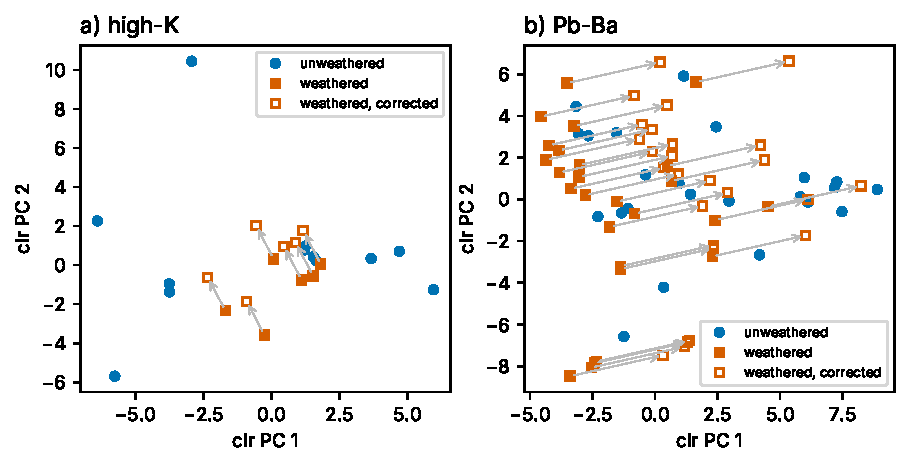
\includegraphics[width=\textwidth]{q1_clr_correction}
\caption{Weathered points before (filled squares) and after (open squares) the clr shift of \cref{eq:shift}, together with the unweathered points, on the first two principal components of the clr coordinates of each type: a) high-K, b) Pb--Ba.}\label{fig:clrcorr}
\end{figure}

\subsubsection{Predicted Compositions}
\Cref{tab:pred} in the appendix lists the predicted pre-weathering composition of all 32 weathered points.
For the Pb--Ba point 02, for example, the prediction is \ox{SiO_2} 63.0\% (90\% interval 57.5--68.2\%) and PbO 21.3\% (17.4--25.3\%), against measured values of 36.3\% and 47.4\% on the weathered surface.
For the high-K point 07 it is \ox{SiO_2} 79.8\% (68.0--86.0\%) with \ox{K_2O} 0.48\% (0.03--9.05\%): potassium was not detected on this surface, so the model can only say that it was low and very uncertain.
The intervals of high-K glass are generally wide, which reflects the six weathered points from which its correction is estimated.
For the same reason, four high-K points with a residual \ox{K_2O} of 0.6--1.0\% receive predictions of 16--22\% \ox{K_2O}, above the largest value (14.5\%) found on unweathered high-K glass; these values should be read as indicating a potassium-rich original glass, not as precise reconstructions.

\subsection{Model Testing}
Two Pb--Ba artefacts, 49 and 50, carry both a weathered point and an unweathered spot, so for them the truth is partly observed.
We re-estimate every correction without the artefact concerned, predict its unweathered composition from its weathered point and compare the prediction with the measured unweathered spot by the mean absolute error (MAE) over the major oxides \ox{SiO_2}, CaO, \ox{Al_2O_3}, CuO, PbO, BaO and \ox{P_2O_5}.
Besides the calibrated and the plain clr shift, we evaluate the clr shift of medians and an additive shift of the mean percentages, which is the most common approach in contest solutions, and we add a plausibility check that applies to all weathered points: the share of predicted major-oxide values lying inside the range observed on unweathered points of the same type.

\begin{table}[ht]
\centering
\caption{Test of the weathering corrections: MAE (wt\%) of the major oxides and Aitchison distance $d_A$ on the two paired artefacts (leave-one-artefact-out), and plausibility on all weathered points (share of predicted major-oxide values inside the unweathered range; points with all values inside).}\label{tab:val}
\small
\begin{tabular}{lrrrrrrrr}
\toprule
& \multicolumn{2}{c}{Artefact 49} & \multicolumn{2}{c}{Artefact 50} & \multicolumn{2}{c}{High-K (6 points)} & \multicolumn{2}{c}{Pb--Ba (26 points)} \\
\cmidrule(lr){2-3}\cmidrule(lr){4-5}\cmidrule(lr){6-7}\cmidrule(lr){8-9}
Correction & MAE & $d_A$ & MAE & $d_A$ & share & points & share & points \\
\midrule
None & 7.30 & 4.51 & 8.09 & 4.45 & 0.77 & 0 & 0.66 & 1 \\
Additive shift (wt\%) & 2.95 & 7.54 & 3.69 & 7.62 & 1.00 & 6 & 0.90 & 14 \\
clr median shift & 2.81 & 3.77 & 3.63 & 4.77 & 0.90 & 1 & 0.90 & 11 \\
clr mean shift, \cref{eq:shift} & 3.74 & 4.38 & 5.72 & 5.66 & 0.88 & 2 & 0.93 & 16 \\
Calibrated shift, \cref{eq:gain} & 3.40 & 4.35 & 4.62 & 5.44 & 0.90 & 2 & 0.99 & 23 \\
\bottomrule
\end{tabular}
\end{table}

\Cref{tab:val} and \cref{fig:val} show that every correction roughly halves the error of the uncorrected weathered values.
The calibrated shift improves on the plain shift on both artefacts and on both measures, since it no longer over-corrects the major oxides of Pb--Ba glass: for artefact 50 it predicts \ox{SiO_2} 57.9\% and PbO 24.1\% against measured 46.4\% and 31.6\%, whereas the plain shift predicts BaO 26.2\% against a measured 6.4\%.
It is also the most plausible correction for Pb--Ba glass, with 98.6\% of the predicted values and 23 of the 26 points inside the unweathered range.
The additive shift and the median shift reach a slightly lower MAE on the two artefacts, but with only two test artefacts these differences are within the variation between artefacts.
The additive shift, moreover, pays for its MAE with by far the largest Aitchison distances, because subtracting average percentages drives minor oxides to zero or below, and the median shift is less plausible, markedly so for Pb--Ba glass, since medians of clr coordinates are unstable for parts that are undetected in about half of the points.
The Aitchison distance, which weights all 14 parts equally, is hardly improved by any correction and is even slightly worse than without correction for artefact 50; it is dominated by trace oxides near the detection limit, whose original values cannot be recovered from a weathered surface, and on it too the calibrated shift does better than the plain shift.
We therefore keep the calibrated shift, which is derived from an explicit model, improves on the plain shift on every criterion, is the most plausible correction for Pb--Ba glass and comes close to the lowest MAE.

\begin{figure}[ht]
\centering
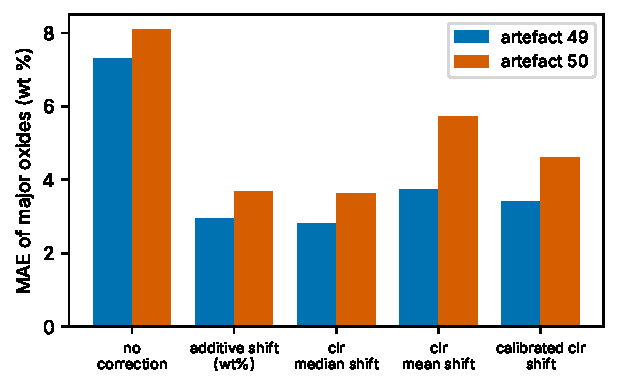
\includegraphics[width=0.62\textwidth]{q1_prediction_validation}
\caption{MAE of the major oxides between the corrected weathered point and the unweathered spot of artefacts 49 and 50 for five corrections, each estimated without the artefact itself.}\label{fig:val}
\end{figure}

The paired and severely weathered spots also allow a check of the direction of weathering assumed in \cref{eq:model}.
If weathering followed the average direction $-\hat\Delta$ exactly, the clr difference between a weathered point and an unweathered spot of the same artefact would be parallel to it.
The cosines between the observed differences and $-\hat\Delta_{\text{Pb--Ba}}$ are 0.49 for artefact 49 and 0.15 for artefact 50, and those between the severely weathered and the regular weathered point of artefacts 08, 26 and 54 are 0.40, $-0.08$ and 0.10.
In 13 dimensions, 95\% of random directions have a cosine below 0.53 in absolute value, so the individual weathering paths are only loosely aligned with the average direction.
This is precisely the artefact-specific deviation $e$ of \cref{eq:model}; it explains why the plain shift over-corrects and why the gains of the calibrated shift are useful, and it limits the accuracy that any correction estimated from unpaired data can reach.

%% ================================================================== 6
\section{Model II: Classification Rule and Sub-Classes (Problem 2)}\label{sec:q2}

\subsection{Classification Rule}

\subsubsection{Separability of Single Oxides}
A classification rule should be simple, chemically meaningful and valid for weathered as well as unweathered glass.
Since the two types are defined by their flux, we first examine the raw percentage of each oxide and of the sum PbO+BaO, and measure how well a single threshold separates the 67 valid points.
For a variable with high-K range $[a_1,a_2]$ and Pb--Ba range $[b_1,b_2]$, the gap $b_1-a_2$ is positive if and only if the variable separates the types without error, and its size is the margin of the rule.

\begin{table}[ht]
\centering
\caption{Separation of the types by single variables on the 67 valid points (wt\%). The gap is $\min_{\text{Pb--Ba}}-\max_{\text{high-K}}$ (or the reverse); the accuracy is that of the best single threshold.}\label{tab:sep}
\small
\begin{tabular}{lrrrrrr}
\toprule
Variable & high-K min & high-K max & Pb--Ba min & Pb--Ba max & gap & accuracy \\
\midrule
PbO+BaO & 0.00 & 4.27 & 14.34 & 76.90 & 10.07 & 1.000 \\
PbO & 0.00 & 1.62 & 9.30 & 70.21 & 7.68 & 1.000 \\
BaO & 0.00 & 2.86 & 0.00 & 35.45 & $-2.86$ & 0.940 \\
\ox{K_2O} & 0.00 & 14.52 & 0.00 & 1.41 & $-1.41$ & 0.910 \\
\ox{SiO_2} & 59.01 & 96.77 & 3.72 & 75.51 & $-16.50$ & 0.866 \\
SrO & 0.00 & 0.12 & 0.00 & 1.12 & $-0.12$ & 0.851 \\
\bottomrule
\end{tabular}
\end{table}

\Cref{tab:sep} shows that only lead separates the types.
The sum PbO+BaO is at most 4.27\% on every high-K point and at least 14.34\% on every Pb--Ba point, weathered or not, a gap of ten percentage points; PbO alone also separates them, with a smaller gap of 7.7 points.
BaO fails because three weathered Pb--Ba points have lost their barium, and \ox{K_2O} fails because potassium is not detected on two weathered high-K points and on the unweathered point 21, which is the reason why the defining flux of high-K glass cannot serve as a rule.
Placing the threshold in the middle of the gap gives the rule
\begin{equation}\label{eq:rule}
\text{type}(x)=\begin{cases}\text{Pb--Ba}, & x_{\mathrm{PbO}}+x_{\mathrm{BaO}} > 9.3\%,\\ \text{high-K}, & \text{otherwise},\end{cases}
\end{equation}
whose chemical meaning is that lead ore is the flux of Pb--Ba glass, and that weathering, which enriches lead, can only increase the margin of Pb--Ba points.

\subsubsection{Multivariate Confirmation}
To check that the rule does not overlook information in the other oxides, we fit three classifiers and validate them by leave-one-artefact-out cross-validation, in which all points of one artefact are removed together, the model is fitted to the rest and the removed points are predicted.
A classification tree of depth two \citep{breiman1984} on the raw percentages places its first split at PbO $\le 5.46\%$, inside the gap of \cref{tab:sep}, and classifies all 67 points correctly in validation.
A random forest of 500 trees \citep{breiman2001} also classifies all points correctly, and its impurity importances rank PbO (0.31), BaO (0.19), \ox{SiO_2} (0.13), \ox{K_2O} (0.11) and SrO (0.10) highest.
An $\ell_2$-regularised logistic regression on the 14 clr coordinates, finally, classifies 66 of 67 points correctly; its largest coefficients are $+1.20$ for clr(PbO), $+0.43$ for clr(SrO) and $-0.42$ for clr(CuO), and its only error is point 21, the high-K point without detected \ox{K_2O}, whose PbO+BaO of 2.97\% is nevertheless clearly classified by the rule.
All three methods therefore point to lead as the decisive variable, and the rule \cref{eq:rule} is as accurate as the more complex models while being directly interpretable.

\subsection{Sub-Class Model}
Within each type, sub-classes should reflect differences in recipe or raw materials, not differences in weathering, so we cluster the weathering-corrected clr coordinates, $z+\hat\Delta_t$ for weathered points.
Here we use the plain shift rather than the calibrated shift, because the gains of the calibrated shift pull weathered points towards the centre of their type and would therefore compress exactly the differences that a clustering is meant to find.
For each type, six oxides that carry its chemical variation are used: \ox{K_2O}, CaO, \ox{Al_2O_3}, \ox{Fe_2O_3}, CuO and \ox{SiO_2} for high-K glass, and PbO, BaO, \ox{SiO_2}, CuO, \ox{P_2O_5} and \ox{Al_2O_3} for Pb--Ba glass; the coordinates are standardised to unit variance so that each oxide has equal weight.

We use Ward's hierarchical clustering \citep{ward1963}, which merges at each step the two clusters whose union increases the within-cluster sum of squares
\begin{equation}
W_k=\sum_{c=1}^{k}\sum_{i\in c}\lVert z_i-\bar z_c\rVert^2
\end{equation}
least, and which therefore produces compact clusters that can be described by their mean compositions.
The number of clusters $k\in\{2,\dots,5\}$ is chosen to maximise the mean silhouette \citep{rousseeuw1987},
\begin{equation}
s(i)=\frac{b(i)-a(i)}{\max\{a(i),b(i)\}},
\end{equation}
where $a(i)$ is the mean distance of point $i$ to the other members of its cluster and $b(i)$ the smallest mean distance to another cluster, subject to the requirement that every cluster contains at least three points, so that a sub-class is more than an isolated pair of measurements.

\subsection{Sub-Class Results}
For Pb--Ba glass the mean silhouette is 0.213, 0.252, 0.280 and 0.275 for $k=2,3,4,5$, so four sub-classes are chosen.
\Cref{tab:sub} describes them by the median of their weathering-corrected compositions, which removes the weathering signal from the medians and makes the chemical differences visible.
The two large sub-classes contain points of both weathering states.
Sub-class 4, with 18 points, is a low-impurity glass in which \ox{P_2O_5}, MgO and \ox{Fe_2O_3} are close to the detection limit, whereas sub-class 2, with 24 points, contains measurable amounts of these impurities (\ox{P_2O_5} 0.56\%, MgO 0.75\%, \ox{Fe_2O_3} 0.32\%) together with the lowest PbO.
Sub-class 1 consists of four high-lead points (PbO 38.9\%) without detectable copper, and sub-class 3 of three barium-free points (BaO not detected) with the highest \ox{Al_2O_3}.
Each sub-class is thus characterised by one or two oxides with a clear interpretation in terms of raw materials, namely the purity of the silica and lead sources, the use of barium and the addition of copper as a colourant.
All three members of sub-class 3 are weathered, however, and one of them is a severely weathered spot, so the absence of barium may partly be a weathering effect that the average correction does not remove.

\begin{table}[ht]
\centering
\caption{Pb--Ba sub-classes: size, weathered members and median weathering-corrected composition (wt\%) of selected oxides.}\label{tab:sub}
\small
\begin{tabular}{lrrrrrrrrrr}
\toprule
Sub-class & $n$ & weath. & \ox{SiO_2} & PbO & BaO & CuO & \ox{Al_2O_3} & \ox{P_2O_5} & MgO & \ox{Fe_2O_3} \\
\midrule
1, copper-free & 4 & 2 & 41.52 & 38.85 & 10.49 & 0.00 & 4.18 & 0.10 & 0.76 & 1.26 \\
2, impurity-bearing & 24 & 14 & 53.83 & 18.08 & 10.80 & 0.85 & 3.95 & 0.56 & 0.75 & 0.32 \\
3, barium-free & 3 & 3 & 59.81 & 29.62 & 0.01 & 0.50 & 7.28 & 0.76 & 1.94 & 0.31 \\
4, low-impurity & 18 & 7 & 58.68 & 18.58 & 11.20 & 0.54 & 2.44 & 0.02 & 0.01 & 0.01 \\
\bottomrule
\end{tabular}
\end{table}

For high-K glass, no partition into clusters of at least three points exists for $k\le5$.
The best unconstrained partition, with a silhouette of 0.48 at $k=2$, separates two unweathered points (03 part~1 and 18), which are richer in silica and poorer in CaO than the rest, from the other 16; with only two members, it describes two unusual measurements rather than a sub-class.
\Cref{fig:dendro} shows the dendrograms, in which the high-K tree has no level at which it divides into groups of comparable size, while the Pb--Ba tree has three upper merges that lie well above all others.
\Cref{fig:sub} shows the resulting sub-classes on the first two principal components.

\begin{figure}[ht]
\centering
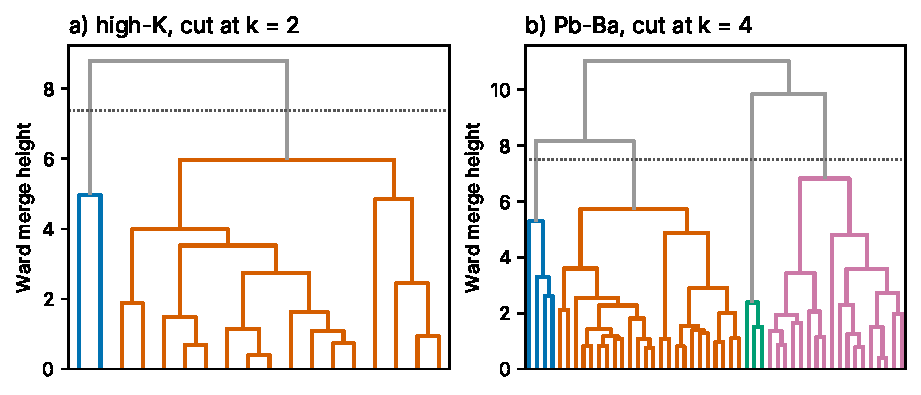
\includegraphics[width=\textwidth]{q2_dendrograms}
\caption{Ward dendrograms of the standardised, weathering-corrected clr coordinates: a) high-K (18 points), b) Pb--Ba (49 points). The dotted line marks the cut that gives the chosen number of clusters.}\label{fig:dendro}
\end{figure}

\begin{figure}[ht]
\centering
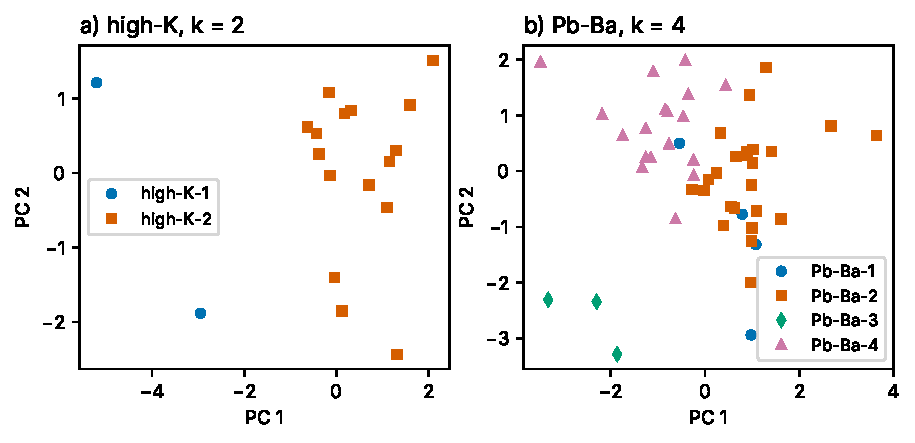
\includegraphics[width=\textwidth]{q2_subclasses}
\caption{Sub-classes from Ward clustering on the first two principal components of the standardised, weathering-corrected clr coordinates: a) high-K, b) Pb--Ba.}\label{fig:sub}
\end{figure}

\subsection{Rationality of the Division}
A division is rational if it does not depend on the particular algorithm and if the data contain a structure that it describes.
For the first point, we compare the Ward partition with four alternatives at the same $k$ by the adjusted Rand index \citep{hubert1985}, which is 1 for identical partitions and close to 0 for unrelated ones (\cref{tab:rat}).
k-means reproduces the Ward partition exactly in both types and complete linkage almost exactly (ARI 0.95 for Pb--Ba glass), whereas average linkage and a Gaussian mixture with diagonal covariances split off single points and agree less.
Clustering on all 14 clr coordinates instead of six oxides gives a quite different partition of Pb--Ba glass (ARI 0.33), because the eight additional coordinates are mostly trace oxides near the detection limit, whose replaced values add noise; this is why we cluster on the oxides that carry the chemistry of each type.

\begin{table}[ht]
\centering
\caption{Agreement (ARI) of alternative clusterings with the Ward partition, and the smallest cluster of each alternative.}\label{tab:rat}
\small
\begin{tabular}{lrrrr}
\toprule
& \multicolumn{2}{c}{High-K ($k=2$)} & \multicolumn{2}{c}{Pb--Ba ($k=4$)} \\
\cmidrule(lr){2-3}\cmidrule(lr){4-5}
Alternative & ARI & smallest & ARI & smallest \\
\midrule
k-means (50 starts) & 1.00 & 2 & 1.00 & 3 \\
Complete linkage & 1.00 & 2 & 0.95 & 3 \\
Average linkage & 0.59 & 1 & 0.19 & 1 \\
Gaussian mixture (diagonal) & 0.59 & 1 & 0.68 & 1 \\
Ward, all 14 clr coordinates & 0.59 & 1 & 0.33 & 5 \\
\bottomrule
\end{tabular}
\end{table}

For the second point, we use the gap statistic \citep{tibshirani2001}, which compares $\log W_k$ with its expectation under 100 reference data sets drawn uniformly from the box spanned by the principal components of the data, and selects the smallest $k$ with $\text{Gap}(k)\ge\text{Gap}(k+1)-s_{k+1}$.
For both types this rule selects $k=1$.
For Pb--Ba glass the gap first falls from 0.60 at $k=1$ to 0.52 at $k=2$ and then rises to 0.62 at $k=4$ and 0.65 at $k=5$, with a standard error of about 0.07, so a structure at four clusters exists but is weak, and the mean silhouette of 0.28 points in the same direction.
The Pb--Ba sub-classes are therefore best understood as a consistent partition of a graded compositional variation, in which the four groups are located in different parts of a continuum and are not separated by empty regions.
For high-K glass, the data support no sub-classes at all.

\subsection{Sensitivity of the Division}
We measure the sensitivity of the sub-classes by the ARI between the reference partition and partitions of perturbed data.
Three perturbations are used: bootstrap resampling of the points of a type (200 resamples), multiplicative measurement noise, for which every percentage is multiplied by $e^{\varepsilon Z}$ with $Z\sim N(0,1)$ and $\varepsilon\in\{2,5,10,20\}\%$ (100 draws each), and the omission of the weathering correction.
The Pb--Ba sub-classes are stable to measurement noise, with a mean ARI of 0.98, 0.96, 0.91 and 0.82 at the four noise levels, but only moderately stable to resampling (median ARI 0.75, 10th percentile 0.39), which is consistent with a partition of a continuum, whose boundaries move when the points near them are resampled.
Without weathering correction the partition changes substantially (ARI 0.40), so the correction is an essential step of the division.
The best high-K split has a bootstrap 10th-percentile ARI of 0, which confirms that it is not reproducible.
Further sensitivities, to the detection-limit replacement and to the correction model, are reported in \cref{sec:sens}.

%% ================================================================== 7
\section{Model III: Identification of Unknown Artefacts (Problem 3)}\label{sec:q3}

\subsection{Classification Models}
The eight unclassified artefacts are identified with three methods of increasing complexity.
The first is the rule \cref{eq:rule}.
The second is the logistic model of \cref{sec:q2}, fitted to all 67 valid points, which gives a probability of Pb--Ba glass.
The third is a nearest-centre classifier in Aitchison geometry: the composition of an unknown artefact is corrected for weathering under each type hypothesis, if it is weathered, and the artefact is assigned to the type whose corrected clr centre is closer.
The third method uses all oxides and the weathering status, so it tests the assignment with information that the rule ignores.

Artefacts assigned to Pb--Ba glass are also placed in a sub-class.
Their weathering-corrected clr coordinates of the six Pb--Ba oxides are standardised with the means and standard deviations of the labelled Pb--Ba points, and the artefact is assigned to the nearest sub-class centre; the ratio of the distances to the nearest and the second-nearest centre measures how clear the assignment is, a ratio near one meaning that the artefact lies between two sub-classes.

\subsection{Results}
\Cref{tab:unk} shows that the three methods agree on every artefact: A1, A6 and A7 are high-K glass and A2, A3, A4, A5 and A8 are Pb--Ba glass.
The Aitchison distances are clear-cut for all artefacts except A5, whose distance to the Pb--Ba centre (7.77) is not much smaller than that to the high-K centre (9.75).
A5 is also the least certain case of the other methods.
It is weathered, its PbO+BaO of 14.39\% is just above the smallest value of the labelled Pb--Ba points, and its logistic probability of 0.94 is the lowest of the five Pb--Ba assignments; its high \ox{SiO_2} (64.3\%) and \ox{Al_2O_3} (12.8\%) make it a Pb--Ba glass with relatively little lead.
A1 contains neither \ox{K_2O} nor PbO and BaO above detection, so it is assigned to high-K glass because it lacks the Pb--Ba signature rather than because it shows the high-K flux, like the labelled point 21.

\begin{table}[ht]
\centering
\setlength{\tabcolsep}{4.5pt}
\caption{Identification of the unclassified artefacts. $p$ is the logistic probability of Pb--Ba glass, $d_{\mathrm K}$ and $d_{\mathrm P}$ are Aitchison distances to the corrected type centres, and the distance ratio refers to the nearest and second-nearest Pb--Ba sub-class.}\label{tab:unk}
\small
\begin{tabular}{lcrrrrrlll}
\toprule
Artefact & weath. & PbO+BaO & \ox{K_2O} & $p$ & $d_{\mathrm K}$ & $d_{\mathrm P}$ & type & sub-class & ratio \\
\midrule
A1 & no & 0.00 & 0.00 & 0.000 & 8.82 & 13.64 & high-K & -- & -- \\
A2 & yes & 34.30 & 0.00 & 0.999 & 12.88 & 9.11 & Pb--Ba & 3, barium-free & 0.60 \\
A3 & no & 44.27 & 1.36 & 0.985 & 9.16 & 7.22 & Pb--Ba & 2, impurity-bearing & 0.73 \\
A4 & no & 32.59 & 0.79 & 0.955 & 8.79 & 6.90 & Pb--Ba & 2, impurity-bearing & 0.50 \\
A5 & yes & 14.39 & 0.37 & 0.943 & 9.75 & 7.77 & Pb--Ba & 2, impurity-bearing & 0.91 \\
A6 & yes & 0.00 & 1.35 & 0.000 & 2.86 & 12.23 & high-K & -- & -- \\
A7 & yes & 0.00 & 0.98 & 0.000 & 3.95 & 12.64 & high-K & -- & -- \\
A8 & no & 32.58 & 0.23 & 0.997 & 12.67 & 8.69 & Pb--Ba & 2, impurity-bearing & 0.52 \\
\bottomrule
\end{tabular}
\end{table}

A2, which has lost its barium and is very rich in \ox{P_2O_5} (14.3\%), falls in the barium-free sub-class.
A3, A4 and A8 contain several percent of \ox{Fe_2O_3} or CuO and fall in the impurity-bearing sub-class, as does A5, although its distance ratio of 0.91 places it close to the boundary with the low-impurity sub-class.

\subsection{Sensitivity of the Identification}
We perturb each unknown composition 2{,}000 times by multiplying every percentage by $e^{\varepsilon Z}$ and record the share of perturbations that leave the logistic assignment unchanged.
For all eight artefacts this share is 100\% at every level up to $\varepsilon=40\%$, which corresponds to relative measurement errors far larger than any plausible error of the chemical analysis.
The rule is equally robust, since the smallest PbO+BaO of an artefact assigned to Pb--Ba glass (A5, 14.39\%) would have to fall by more than a third to cross the threshold of 9.3\%, while the high-K artefacts contain no lead at all.
The sub-class assignments are almost as stable: the same perturbations at $\varepsilon=5$, 10 and 20\% leave them unchanged in all cases except for A5 at 20\%, which keeps its sub-class in 99.8\% of the perturbations.
\Cref{sec:sens} shows, finally, that the type assignments are identical for every detection-limit replacement and every regularisation strength that we examined.

%% ================================================================== 8
\section{Model IV: Associations between Oxides (Problem 4)}\label{sec:q4}

\subsection{Model}
Associations between the parts of a composition can be measured in two complementary ways in log-ratio geometry.
The first is the correlation of clr coordinates, which describes whether two parts rise and fall together relative to the geometric mean of the composition.
The second is the variation matrix \citep{aitchison1986},
\begin{equation}
\tau_{ij}=\operatorname{Var}\big(\log(x_i/x_j)\big)=\operatorname{Var}\big(\clr(x)_i-\clr(x)_j\big),
\end{equation}
which is zero when two parts are exactly proportional and does not depend on the other parts, so a small $\tau_{ij}$ identifies parts that come from the same source in a fixed ratio.
We compute both measures within each type on the weathering-corrected clr coordinates, so that the associations describe the glass rather than its weathering, and restrict them to the 11 oxides detected in at least half of the points, because the log-ratios of rarely detected oxides mainly reflect the replacement value.

The significance of each within-type correlation is tested with the $t$-test of $r$, and the 55 $p$-values of each type are controlled with the Benjamini--Hochberg procedure at a false discovery rate of 5\% \citep{bh1995}.
A difference of a correlation between the types is tested with Fisher's $z$-transform \citep{fisher1915},
\begin{equation}
z = \frac{\operatorname{artanh} r_1 - \operatorname{artanh} r_2}{\sqrt{1/(n_1-3)+1/(n_2-3)}},
\end{equation}
which is approximately standard normal under equal correlations, with $n_1=18$ and $n_2=49$, and these 55 $p$-values are again controlled by the Benjamini--Hochberg procedure.
Because the normal approximation is optimistic for 18 points, we add 95\% bootstrap intervals for the pairs that differ most.

Raw percentages would give a misleading picture.
Among the pairs whose correlation exceeds 0.3 in absolute value on either scale, the sign differs between raw percentages and clr coordinates for 23 of 55 pairs in high-K glass and for 8 in Pb--Ba glass.
In high-K glass, where silica makes up two thirds of the composition, almost every oxide is negatively correlated with \ox{SiO_2} in raw percentages, for example $r=-0.88$ for \ox{K_2O} and $-0.83$ for \ox{Al_2O_3}, simply because a larger share of silica leaves less room for everything else.

\subsection{Associations within Each Type}
In high-K glass, two correlations are significant after false-discovery-rate control.
\ox{SiO_2} and \ox{Fe_2O_3} are negatively associated ($r=-0.76$, $q=0.014$), which suggests that iron entered the glass with the flux or with impure raw materials rather than with the silica, and CaO and SrO are also negatively associated ($r=-0.69$, $q=0.047$).
The variation matrix shows that \ox{SiO_2} and \ox{Al_2O_3} have the most constant ratio of all pairs ($\tau=0.23$), consistent with alumina entering the glass as an impurity of the sand.

In Pb--Ba glass, five correlations are significant.
\ox{SiO_2} and PbO are positively associated ($r=0.61$, $q<0.001$) and have the smallest log-ratio variance of the type ($\tau=0.37$), so that lead and silica occur in a fairly stable ratio, the two main ingredients of the recipe; \ox{SiO_2} and \ox{Al_2O_3} follow ($r=0.42$, $\tau=0.49$).
BaO is negatively associated with MgO ($r=-0.53$) and \ox{Al_2O_3} ($r=-0.42$), and \ox{Fe_2O_3} and CuO are negatively associated ($r=-0.49$, $q=0.007$), which suggests that copper and iron were not supplied by the same material in this glass.

\subsection{Differences between the Types}
\Cref{fig:corr} shows the two correlation matrices and their difference.
After false-discovery-rate control, two of the 55 pairs differ significantly between the types.
The clearest is \ox{Fe_2O_3}--CuO, with $r=0.62$ in high-K and $-0.49$ in Pb--Ba glass ($z=4.22$, $q=0.001$); in high-K glass the two colourants rise together, which points to a common source such as a copper ore containing iron, whereas in Pb--Ba glass they vary in opposite directions.
The second is \ox{SiO_2}--\ox{Fe_2O_3}, with $r=-0.76$ against $-0.01$ ($q=0.024$), and CaO--CuO and CaO--SrO follow at $q=0.06$.

The bootstrap intervals qualify the high-K estimates.
The 95\% interval for \ox{Fe_2O_3}--CuO is $[-0.05,\,0.96]$ in high-K glass against $[-0.66,\,-0.31]$ in Pb--Ba glass, and the interval for \ox{SiO_2}--\ox{Fe_2O_3} in high-K glass is $[-0.92,\,0.08]$.
With 18 points, a few unusual high-K measurements carry much of these correlations, so the difference between the types is firmly established mainly through the precisely estimated Pb--Ba correlations, and most of the other differences in \cref{fig:corr} cannot be resolved with the present data.

\begin{figure}[ht]
\centering
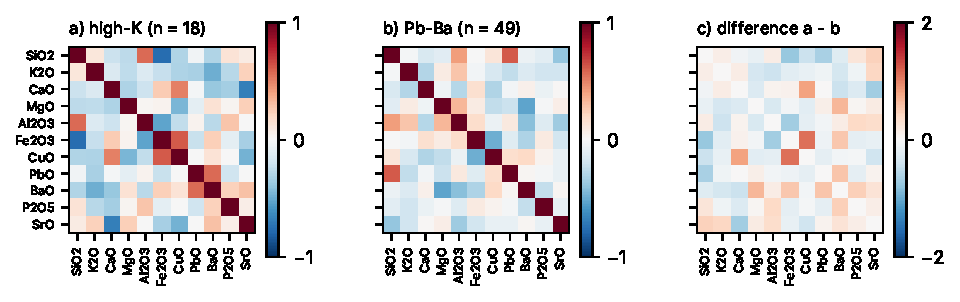
\includegraphics[width=\textwidth]{q4_correlations}
\caption{Pearson correlations of the weathering-corrected clr coordinates of the 11 oxides detected in at least half of the points: a) high-K, b) Pb--Ba, c) difference a$-$b.}\label{fig:corr}
\end{figure}

%% ================================================================== 9
\section{Sensitivity Analysis}\label{sec:sens}

The models contain three choices that are not dictated by the data: the replacement value $\delta$ for undetected oxides, the estimator of the weathering correction and the regularisation strength $C$ of the logistic model.
We repeat the main computations for $\delta\in\{0.001,0.0025,0.005,0.01,0.02\}\%$, for the clr median shift in place of the mean shift and for $C$ from 0.01 to 100, and summarise the results in \cref{tab:sens}.

\begin{table}[ht]
\centering
\caption{Sensitivity of the main results to the detection-limit replacement $\delta$, the correction estimator and the regularisation $C$ (reference: $\delta=0.005\%$, mean shift, $C=1$). MAE: calibrated correction on artefacts 49/50; LOAO: leave-one-artefact-out accuracy of the logistic model; $k$: silhouette-selected number of Pb--Ba sub-classes; ARI: agreement of the Pb--Ba partition at $k=4$ with the reference; Q4: significant type differences.}\label{tab:sens}
\small
\begin{tabular}{lrrrcrrr}
\toprule
Setting & MAE 49 & MAE 50 & LOAO & unknown types & $k$ & ARI & Q4 \\
\midrule
$\delta=0.001\%$ & 3.52 & 4.63 & 0.985 & unchanged & 5 & 1.00 & 4 \\
$\delta=0.0025\%$ & 3.46 & 4.63 & 0.985 & unchanged & 5 & 1.00 & 2 \\
$\delta=0.005\%$ (reference) & 3.40 & 4.62 & 0.985 & -- & 4 & 1.00 & 2 \\
$\delta=0.01\%$ & 3.34 & 4.60 & 0.985 & unchanged & 4 & 0.81 & 3 \\
$\delta=0.02\%$ & 3.27 & 4.57 & 0.985 & unchanged & 3 & 0.43 & 3 \\
\addlinespace
Median shift & -- & -- & 0.985 & unchanged & 5 & 0.95 & 3 \\
\addlinespace
$C=0.01$ & -- & -- & 0.955 & unchanged & -- & -- & -- \\
$C=0.1$ & -- & -- & 0.985 & unchanged & -- & -- & -- \\
$C=10$ & -- & -- & 0.985 & unchanged & -- & -- & -- \\
$C=100$ & -- & -- & 0.985 & unchanged & -- & -- & -- \\
\bottomrule
\end{tabular}
\end{table}

The type assignments are insensitive to all three choices.
The leave-one-artefact-out accuracy is 98.5\% for every $\delta$ and for $C\ge0.1$, and only the strongest regularisation, $C=0.01$, which shrinks all coefficients towards zero, adds two errors; the eight unknown artefacts receive the same types in every setting, and the logistic probability of the least certain artefact, A5, stays between 0.93 and 0.96 across $\delta$ and between 0.79 and 0.99 across $C$.
The weathering correction is also robust: the MAE of the calibrated shift on the paired artefacts varies by less than 0.3 percentage points across a twenty-fold range of $\delta$, while that of the plain shift varies from 3.5 to 3.9 for artefact 49 and from 4.9 to 6.8 for artefact 50, a further advantage of the calibration.

The sub-classes and the associations are more sensitive.
For $\delta\le0.005\%$ the Pb--Ba partition at $k=4$ is identical to the reference, but larger replacement values change it (ARI 0.81 at 0.01\% and 0.43 at 0.02\%), and the silhouette-selected number of sub-classes varies between three and five; the median shift gives almost the same partition (ARI 0.95) but prefers five sub-classes.
These results agree with the weak cluster structure found by the gap statistic: when the data form a continuum, small changes in the geometry move the boundaries and the preferred number of groups.
The number of significant type differences in Problem~4 varies between two and four, but \ox{Fe_2O_3}--CuO and \ox{SiO_2}--\ox{Fe_2O_3} are significant in every setting.
In short, the type rule, the identification of the unknowns and the weathering correction are robust, the Pb--Ba sub-classes are robust in their main features but not in their exact boundaries and number, and the association results beyond these two pairs should be regarded as indicative.

%% ================================================================== 10
\section{Model Evaluation and Further Discussion}\label{sec:evaluation}

\subsection{Strengths}
The models respect the two structural features of the data.
Treating the measurements as compositions removes the closure effects that reverse the sign of many raw-percentage correlations, and working with artefacts as units gives tests and validations with the correct sample size.
The stratified analysis reveals the complete association between decoration B and weathering in high-K glass, which a pooled test misses.
The weathering correction is derived from an explicit model of weathering with artefact-specific deviations, its calibration gains follow from the best linear predictor rather than from tuning, and it is validated on paired spots and checked for plausibility on all weathered points.
The type rule is simple and chemically meaningful, separates the types with a wide margin and is confirmed by three independent classifiers, and every result is accompanied by a test of its sensitivity.

\subsection{Weaknesses}
The weathering correction can be validated on only two Pb--Ba artefacts and not at all for high-K glass, whose correction rests on six weathered points that are all decoration-B artefacts; part of the estimated high-K weathering effect may therefore reflect a difference between decoration-B artefacts and the others, and the high-K predictions of leached components such as \ox{K_2O} are very uncertain.
The diagonal approximation of the calibration ignores correlations between the deviations of different parts.
The replacement of undetected oxides affects the log-ratios of rarely detected parts, which is why the sub-classes and the association analysis are restricted to the oxides that carry most information, and why the Pb--Ba sub-classes depend on the replacement value.
Finally, the Pb--Ba sub-classes partition a continuum, so their boundaries and their number are less certain than their chemical characterisation.

\subsection{Improvements and Extensions}
With more artefacts that carry both weathered and unweathered spots, the covariance of the weathering deviations could be estimated, and a hierarchical model with a random weathering intensity for each artefact would replace the diagonal calibration.
Censored-data methods that treat non-detects as values below a known limit, rather than replacing them, would reduce the sensitivity of the log-ratio analyses to $\delta$.
Model-based clustering on isometric log-ratio coordinates would give a probability of membership in each sub-class, which suits a graded structure better than a hard partition.
The models carry over to other compositional problems in archaeometry and geochemistry, such as the provenance of ceramics or the classification of ores, in which closure, non-detects and alteration of surfaces are equally common.

%% ================================================================== 11
\section{Conclusions}
Surface weathering of these artefacts is associated with glass type, Pb--Ba glass being weathered twice as often as high-K glass, and within high-K glass it coincides completely with decoration B, while colour shows no association.
Weathering leaches potassium and alumina from high-K glass, leaving a silica-rich surface, and depletes silica from Pb--Ba glass while enriching lead, phosphorus and calcium.
A calibrated perturbation model in log-ratio space predicts the pre-weathering composition, halves the error of the uncorrected values on the artefacts where this can be checked and places most corrected Pb--Ba points within the range of unweathered glass.
The types are separated without error by PbO+BaO with a threshold of 9.3\%, the Pb--Ba glass falls into four chemically distinct sub-classes that partition a graded continuum, and the high-K glass has no supported sub-structure.
The eight unknown artefacts are assigned robustly, A1, A6 and A7 to high-K and A2, A3, A4, A5 and A8 to Pb--Ba glass.
Finally, the oxide associations differ between the types most clearly in the \ox{Fe_2O_3}--CuO correlation, which is positive in high-K and negative in Pb--Ba glass and points to different sources of the colourants.

%% ================================================================== References
\begingroup
\small
\begin{thebibliography}{99}
\bibitem[Agresti(2002)]{agresti2002} A.~Agresti. \emph{Categorical Data Analysis}. Wiley, Hoboken, 2nd edition, 2002.
\bibitem[Aitchison(1986)]{aitchison1986} J.~Aitchison. \emph{The Statistical Analysis of Compositional Data}. Chapman and Hall, London, 1986.
\bibitem[Benjamini and Hochberg(1995)]{bh1995} Y.~Benjamini and Y.~Hochberg. Controlling the false discovery rate: a practical and powerful approach to multiple testing. \emph{Journal of the Royal Statistical Society, Series B}, 57(1):289--300, 1995.
\bibitem[Breiman(2001)]{breiman2001} L.~Breiman. Random forests. \emph{Machine Learning}, 45(1):5--32, 2001.
\bibitem[Breiman et~al.(1984)]{breiman1984} L.~Breiman, J.~H. Friedman, R.~A. Olshen, and C.~J. Stone. \emph{Classification and Regression Trees}. Wadsworth, Belmont, 1984.
\bibitem[Fisher(1915)]{fisher1915} R.~A. Fisher. Frequency distribution of the values of the correlation coefficient in samples from an indefinitely large population. \emph{Biometrika}, 10(4):507--521, 1915.
\bibitem[Fuller(1987)]{fuller1987} W.~A. Fuller. \emph{Measurement Error Models}. Wiley, New York, 1987.
\bibitem[Gan(2009)]{gan2009} F.~Gan. Origin and evolution of ancient Chinese glass. In F.~Gan, R.~H. Brill, and S.~Tian, editors, \emph{Ancient Glass Research along the Silk Road}, pages 1--40. World Scientific, Singapore, 2009.
\bibitem[Holm(1979)]{holm1979} S.~Holm. A simple sequentially rejective multiple test procedure. \emph{Scandinavian Journal of Statistics}, 6(2):65--70, 1979.
\bibitem[Hubert and Arabie(1985)]{hubert1985} L.~Hubert and P.~Arabie. Comparing partitions. \emph{Journal of Classification}, 2(1):193--218, 1985.
\bibitem[Mart{\'\i}n-Fern{\'a}ndez et~al.(2003)]{martin2003} J.~A. Mart{\'\i}n-Fern{\'a}ndez, C.~Barcel{\'o}-Vidal, and V.~Pawlowsky-Glahn. Dealing with zeros and missing values in compositional data sets using nonparametric imputation. \emph{Mathematical Geology}, 35(3):253--278, 2003.
\bibitem[Pawlowsky-Glahn et~al.(2015)]{pawlowsky2015} V.~Pawlowsky-Glahn, J.~J. Egozcue, and R.~Tolosana-Delgado. \emph{Modeling and Analysis of Compositional Data}. Wiley, Chichester, 2015.
\bibitem[Rousseeuw(1987)]{rousseeuw1987} P.~J. Rousseeuw. Silhouettes: a graphical aid to the interpretation and validation of cluster analysis. \emph{Journal of Computational and Applied Mathematics}, 20:53--65, 1987.
\bibitem[Tibshirani et~al.(2001)]{tibshirani2001} R.~Tibshirani, G.~Walther, and T.~Hastie. Estimating the number of clusters in a data set via the gap statistic. \emph{Journal of the Royal Statistical Society, Series B}, 63(2):411--423, 2001.
\bibitem[Ward(1963)]{ward1963} J.~H. Ward. Hierarchical grouping to optimize an objective function. \emph{Journal of the American Statistical Association}, 58(301):236--244, 1963.
\end{thebibliography}
\endgroup

%% ================================================================== Appendices
\clearpage
\appendix
\section{Composition Statistics}

\begin{table}[h!]
\centering
\caption{Median composition (wt\%) of the valid points with the detection rate (\%) in parentheses, and Holm-adjusted Mann--Whitney $p$-values for unweathered (U) against weathered (W) points.}\label{tab:compfull}
\small
\begin{tabular}{lrrrrrr}
\toprule
& \multicolumn{3}{c}{High-K (12 U / 6 W)} & \multicolumn{3}{c}{Pb--Ba (23 U / 26 W)}\\
\cmidrule(lr){2-4}\cmidrule(lr){5-7}
Oxide & U & W & $p$ & U & W & $p$ \\
\midrule
SiO$_2$ & 65.53 (100) & 93.50 (100) & 0.002 & 54.61 (100) & 25.02 (100) & $<0.001$ \\
Na$_2$O & 0.00 (25) & 0.00 (0) & 0.882 & 0.00 (43) & 0.00 (15) & 0.116 \\
K$_2$O & 9.83 (92) & 0.67 (67) & 0.050 & 0.15 (65) & 0.00 (35) & 0.879 \\
CaO & 6.10 (83) & 0.83 (100) & 0.249 & 0.84 (87) & 2.88 (96) & 0.023 \\
MgO & 1.17 (83) & 0.00 (33) & 0.163 & 0.71 (65) & 0.57 (58) & 1.000 \\
Al$_2$O$_3$ & 6.19 (100) & 1.72 (100) & 0.003 & 3.86 (100) & 2.38 (100) & 0.218 \\
Fe$_2$O$_3$ & 2.11 (83) & 0.28 (100) & 0.249 & 0.00 (48) & 0.30 (62) & 1.000 \\
CuO & 2.35 (92) & 1.54 (100) & 0.882 & 0.65 (91) & 1.15 (92) & 0.372 \\
PbO & 0.15 (58) & 0.00 (0) & 0.249 & 20.12 (100) & 44.06 (100) & $<0.001$ \\
BaO & 0.00 (33) & 0.00 (0) & 0.696 & 8.99 (100) & 8.79 (88) & 1.000 \\
P$_2$O$_5$ & 1.02 (92) & 0.28 (83) & 0.163 & 0.19 (74) & 4.97 (92) & 0.002 \\
SrO & 0.02 (50) & 0.00 (0) & 0.305 & 0.26 (74) & 0.42 (88) & 0.252 \\
SnO$_2$ & 0.00 (8) & 0.00 (0) & 0.882 & 0.00 (13) & 0.00 (8) & 1.000 \\
SO$_2$ & 0.00 (25) & 0.00 (0) & 0.882 & 0.00 (4) & 0.00 (15) & 1.000 \\
\bottomrule
\end{tabular}
\end{table}

\section{Predicted Pre-Weathering Compositions}

\begingroup
\small
\setlength{\tabcolsep}{5pt}
\begin{longtable}{llrrrrrrrr}
\caption{Predicted pre-weathering composition (wt\%) of the 32 weathered points by the calibrated shift; K denotes high-K glass and ``sev'' a severely weathered spot. Values below 0.05\% correspond to oxides not detected on the weathered surface, which a multiplicative model cannot restore. The full predictions with 90\% bootstrap intervals for all 14 oxides are in \texttt{results/q1\_pre\_weathering\_predictions.csv}.}\label{tab:pred}\\
\toprule
Point & type & \ox{SiO_2} & \ox{K_2O} & CaO & \ox{Al_2O_3} & CuO & PbO & BaO & \ox{P_2O_5} \\
\midrule
\endfirsthead
\toprule
Point & type & \ox{SiO_2} & \ox{K_2O} & CaO & \ox{Al_2O_3} & CuO & PbO & BaO & \ox{P_2O_5} \\
\midrule
\endhead
\bottomrule
\endfoot
02 & Pb--Ba & 63.03 & 3.00 & 0.67 & 5.73 & 0.14 & 21.30 & 3.36 & 0.25 \\
07 & K & 79.83 & 0.48 & 3.21 & 8.48 & 3.76 & 0.08 & 0.04 & 3.33 \\
08 & Pb--Ba & 58.95 & 0.02 & 0.52 & 3.17 & 6.81 & 18.98 & 10.98 & 0.30 \\
08-sev & Pb--Ba & 45.57 & 0.02 & 1.52 & 4.05 & 2.82 & 28.74 & 15.88 & 0.88 \\
09 & K & 72.88 & 15.88 & 1.66 & 5.03 & 1.60 & 0.07 & 0.04 & 1.70 \\
10 & K & 74.49 & 19.88 & 0.56 & 3.10 & 0.87 & 0.07 & 0.04 & 0.02 \\
11 & Pb--Ba & 65.53 & 0.56 & 0.94 & 4.00 & 2.47 & 15.14 & 9.81 & 0.61 \\
12 & K & 67.52 & 22.13 & 1.80 & 5.19 & 1.59 & 0.07 & 0.03 & 0.68 \\
19 & Pb--Ba & 61.74 & 0.01 & 0.77 & 4.61 & 1.74 & 20.42 & 8.68 & 0.56 \\
22 & K & 59.73 & 17.54 & 3.74 & 11.24 & 0.48 & 0.06 & 0.03 & 0.86 \\
26 & Pb--Ba & 58.87 & 0.02 & 0.52 & 2.27 & 7.20 & 19.63 & 10.89 & 0.28 \\
26-sev & Pb--Ba & 43.46 & 1.65 & 1.25 & 4.21 & 2.80 & 27.03 & 18.48 & 0.61 \\
27 & K & 76.55 & 0.49 & 2.70 & 10.29 & 1.71 & 0.08 & 0.04 & 1.88 \\
34 & Pb--Ba & 64.09 & 0.85 & 0.27 & 3.08 & 0.96 & 22.52 & 7.71 & 0.03 \\
36 & Pb--Ba & 57.67 & 0.38 & 0.10 & 2.60 & 0.34 & 17.73 & 7.02 & 0.00 \\
38 & Pb--Ba & 57.44 & 0.01 & 0.20 & 3.60 & 0.40 & 21.14 & 7.40 & 0.03 \\
39 & Pb--Ba & 59.00 & 0.02 & 0.55 & 1.85 & 0.82 & 30.55 & 6.56 & 0.14 \\
40 & Pb--Ba & 52.81 & 0.03 & 1.04 & 1.90 & 0.01 & 36.26 & 6.88 & 0.24 \\
41 & Pb--Ba & 56.03 & 1.04 & 1.18 & 4.71 & 0.09 & 21.63 & 11.37 & 0.43 \\
43-part1 & Pb--Ba & 48.44 & 0.02 & 2.01 & 4.27 & 3.85 & 30.23 & 8.89 & 0.00 \\
43-part2 & Pb--Ba & 58.45 & 0.01 & 1.75 & 4.81 & 0.77 & 22.32 & 9.00 & 0.85 \\
48 & Pb--Ba & 68.13 & 0.51 & 0.45 & 7.58 & 0.00 & 8.81 & 9.30 & 0.04 \\
49 & Pb--Ba & 62.03 & 0.01 & 1.14 & 5.73 & 0.33 & 17.76 & 9.33 & 0.67 \\
50 & Pb--Ba & 57.61 & 0.02 & 1.04 & 3.81 & 0.70 & 24.40 & 10.72 & 0.50 \\
51-part1 & Pb--Ba & 60.17 & 0.01 & 0.78 & 5.68 & 0.56 & 19.30 & 10.94 & 0.43 \\
51-part2 & Pb--Ba & 57.18 & 0.02 & 2.41 & 4.49 & 0.66 & 28.17 & 3.15 & 0.99 \\
52 & Pb--Ba & 57.90 & 0.01 & 0.56 & 2.49 & 0.32 & 21.16 & 9.42 & 0.34 \\
54 & Pb--Ba & 56.62 & 0.90 & 0.90 & 5.19 & 0.44 & 24.81 & 9.09 & 0.29 \\
54-sev & Pb--Ba & 52.29 & 0.03 & 0.00 & 5.72 & 1.45 & 32.41 & 2.84 & 1.97 \\
56 & Pb--Ba & 62.17 & 0.03 & 0.67 & 3.81 & 0.82 & 25.17 & 6.89 & 0.34 \\
57 & Pb--Ba & 58.55 & 0.03 & 0.91 & 4.33 & 1.51 & 28.35 & 6.19 & 0.00 \\
58 & Pb--Ba & 62.68 & 0.74 & 0.76 & 4.42 & 1.28 & 18.41 & 10.04 & 0.47 \\
\end{longtable}
\endgroup

\section{Programs}
All results are computed by the Python program \texttt{code/run\_all.py} with the fixed seeds 2022 and 2023; it reads the contest data from \texttt{data/attachment.xlsx}, runs in about one minute and writes every table and figure of this paper to \texttt{results/}.

\begin{center}
\small
\begin{tabular}{ll}
\toprule
Output file in \texttt{results/} & Content \\
\midrule
\texttt{q1\_association.csv} & \cref{tab:assoc}, pooled tests \\
\texttt{q1\_association\_by\_type.csv} & \cref{tab:assoc}, stratified tests \\
\texttt{q1\_composition\_stats.csv} & \cref{tab:comp,tab:compfull}, \cref{fig:box} \\
\texttt{q1\_centre\_test.csv} & permutation test of clr centres \\
\texttt{q1\_clr\_shift.csv}, \texttt{q1\_calibration.csv} & shifts $\hat\Delta_t$, means and gains $b_{t,j}$ \\
\texttt{q1\_pre\_weathering\_predictions.csv} & \cref{tab:pred} with 90\% intervals \\
\texttt{q1\_correction\_models.csv} & \cref{tab:val} (paired artefacts), \cref{fig:val} \\
\texttt{q1\_correction\_plausibility.csv} & \cref{tab:val} (plausibility) \\
\texttt{q1\_weathering\_direction.csv} & direction check of \cref{eq:model} \\
\texttt{q2\_separability.csv} & \cref{tab:sep} \\
\texttt{q2\_random\_forest\_importance.csv} & forest importances \\
\texttt{q2\_subclasses.csv} & memberships, \cref{fig:dendro,fig:sub} \\
\texttt{q2\_subclass\_profiles\_corrected\_Pb-Ba.csv} & \cref{tab:sub} \\
\texttt{q2\_rationality.csv} & \cref{tab:rat} \\
\texttt{q2\_gap\_statistic.csv} & gap statistic \\
\texttt{q2\_sensitivity.csv} & noise stability of the sub-classes \\
\texttt{q3\_unknown\_classification.csv} & \cref{tab:unk}, rule and logistic model \\
\texttt{q3\_unknown\_subclass.csv} & \cref{tab:unk}, distances and sub-classes \\
\texttt{q4\_within\_type\_pairs.csv} & within-type associations \\
\texttt{q4\_correlation\_differences.csv} & type differences, \cref{fig:corr} \\
\texttt{q4\_bootstrap\_intervals.csv} & bootstrap intervals \\
\texttt{q5\_sensitivity\_delta\_C.csv} & \cref{tab:sens} \\
\texttt{results.json} & counts, rule margins, summary statistics \\
\bottomrule
\end{tabular}
\end{center}

\end{document}
